\chapter{Introduction}

The openSUSE KIWI Image System provides a complete operating system
image solution for Linux supported hardware platforms as well as
for virtualisation systems like Xen. The KIWI architecture was designed
as a two level system. The first stage, based on a valid
\textbf{software package source}, creates a so called \textbf{physical extend}
according to the provided image description. The second stage creates from
a required physical extend an operating system image. The result of the
second stage is called a \textbf{logical extend} or short an image.

\begin{figure}[h]
\centering
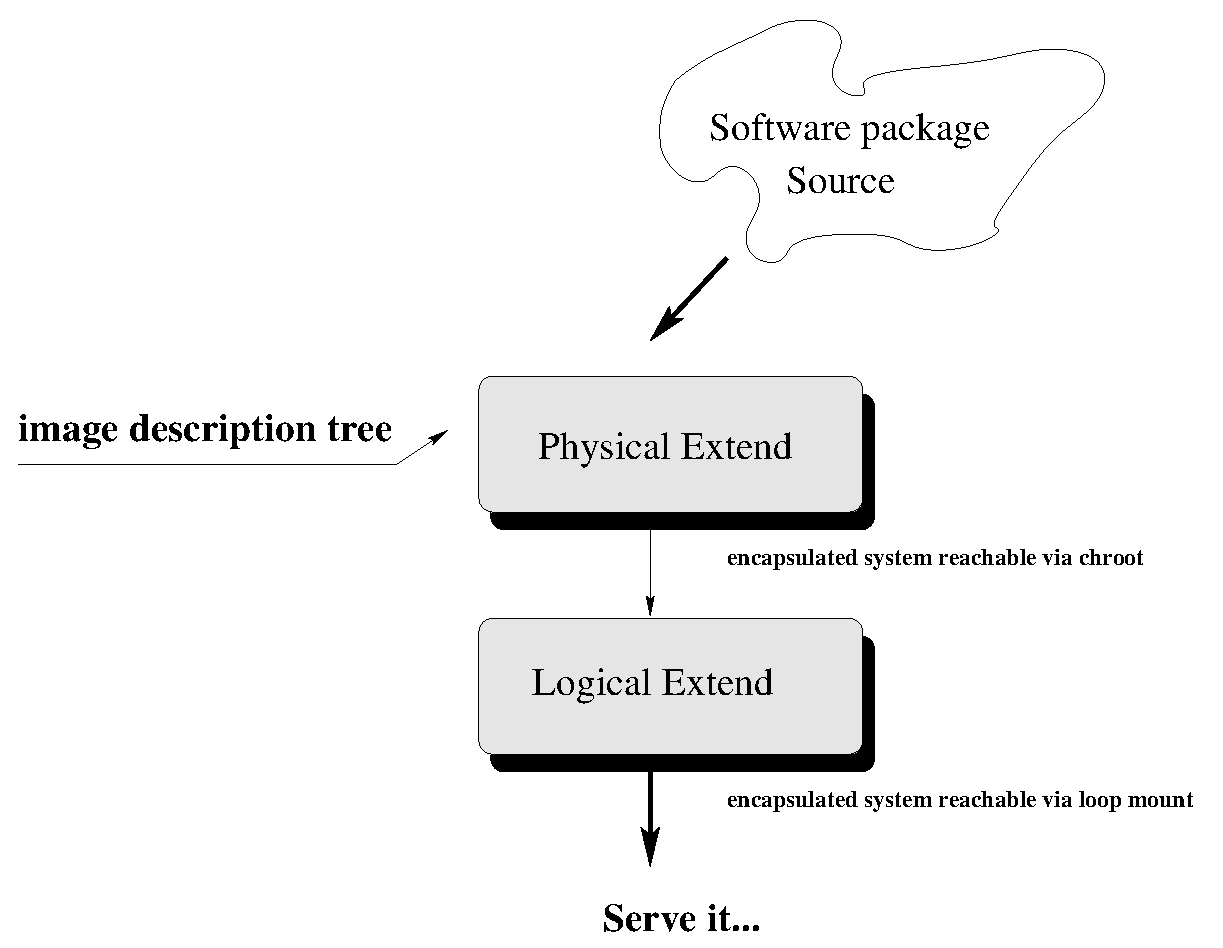
\includegraphics[scale=0.5]{pictures/intro.eps}
\caption{Image Serving Architecture}
\label{fig:architecture}
\end{figure}

Because this document contains conceptual information about an image system,
it is important to understand what an operating system image is all about.
A normal installation process is starting from a given installation source
and installs single pieces of software until the system is complete. During
this process there may be manual user intervention required. However an
operating system image represents an already completed \textit{installation}
encapsulated as a file and optionally includes the configuration for a
specific task. Such an operating system starts working as soon as the
image has been brought to a system storage device no matter if this is a
volatile or non volatile storage. The process of creating an image takes
place without user interaction.
This means all requirements of the encapsulated system has to be fulfilled
before the image is created. According to this the so called
\textbf{image description tree} stores all the information needed to
create an image.

%\newpage

\section{What is KIWI good for}
The solution introduced in this document covers an implementation
for the following two major topics:

\begin{itemize}
	\item How to create physical and logical extends
	\item How to serve/activate a logical extend, an image
\end{itemize}

As already said a physical extend requires a valid software package
source. This is the location where KIWI can access the software to
build up a system. Software exists as packages and packages exists
in different formats. The amount of all packages are organized in
a package tree including some meta data, this is called a repository.
With the KIWI project I want to be free of choice what kind of
package repository should be used. To achieve this goal this project
will make use of the \textbf{smart} package manager which is very
fast and can handle the most important repository structures.
Information on smart can be found here:

\begin{itemize}
	\item http://labix.org/smart
\end{itemize}

\subsection{Supported image types}
To create a logical extend it is necessary to create a filesystem
the operating system data can be stored in. The image type corresponds
to the selected filesystem. Supported image types are:

\begin{itemize}
	\item \textbf{\underline{CPIO}}
	\item \textbf{\underline{EXT2 / EXT3}}
	\item \textbf{\underline{ReiserFS}}
	\item \textbf{\underline{CramFS}}\\
		  for read-only part of \textbf{split} images only
	\item \textbf{\underline{Special cpio/ext2 Boot image}}\\
          for image installation via network
	\item \textbf{\underline{Special cpio/ext2 XEN-Boot image}}\\
          based on Xen kernel and mboot.c32 for multiboot of xen plus
		  initrd (kiwi boot image).
	\item \textbf{\underline{Special cpio/ext2 ISO-Boot image}}\\
          to create a kiwi boot image for booting a live CD 
          system image. Used in combination with the \textbf{iso:}
          image type 
	\item \textbf{\underline{Special cpio/ext2 USB-Boot image}}\\
          to create a kiwi boot image for booting a USB stick
          system image. Used in combination with the
          \textbf{usb:} image type
	\item \textbf{\underline{Special cpio/ext2 VMX-Boot image}}\\
          to create a kiwi boot image for booting a virtual
          machine system image. This is \textbf{not} used for paravirtualized
	      machines like Xen but for full virtual machines like
          QEMU and VMware. Used in combination with the \textbf{vmx:}
          image type
	\item \textbf{\underline{iso:<boot-image-name> image support}}\\
          LiveCD/DVD system image, which means the image gets
          splitted into two ext2 based sub-images whereas one represents
          the loop read-only part on CD and the other represents the
          read-write data in RAM
	\item \textbf{\underline{usb:<fstype>:<boot-image-name>}}\\
          USB stick system image, which means the system image and
          the boot image will be created automatically. To deploy the
          image on the stick the --bootstick option can be used
	\item \textbf{\underline{vmx:<fstype>:<boot-image-name>}}\\
          Virtual machine system image, which means a virtual disk will
          be created including boot manager boot image and system image
          to be used within qemu (.qemu file) or vmware player (.vmdk file)
    \item \textbf{\underline{xen:<fstype>:<boot-image-name>}}\\
          Xen machine system image, which means an image plus boot image will
          be created including the Xen configuration to start the image.
	\item \textbf{\underline{pxe:<fstype>:<boot-image-name>}}\\
          PXE system image, which means an image plus boot image will
          be created. Additionally one can add a deploy section into the
          config.xml which is used to created the config.<MAC> file for
          the pxe network deployment of this image
	\item \textbf{\underline{split:<fstypeRW,fstypeRO> image support}}\\
          Which means the image is splitted into a read-only and a
          read-write part whereas each part can have a different
          filesystem. To be able to boot such an image the config.<MAC>
          file must contain a \textit{COMBINED\_IMAGE=yes} statement.
\end{itemize}
